\documentclass[english,twoside,9pt]{extarticle}
% Author: 
%
%	Oliver Sheridan-Methven, November 2017.
%	
% Description:
%
%	A collection of extremely useful packages 
%	which have been accumulated over a long time,
%	all of which combine to make very nice LaTeX
%	documents. 



\usepackage{adjustbox} % Nice alternative to minipage.
\usepackage{afterpage} % To give the title page its own geometry.
\usepackage{amsmath} % Nice maths symbols.
\usepackage{amssymb} % Nice variable symbols.
\usepackage{array} % Allow for custom column widths in tables.
\usepackage{ltablex} % For long tables spanning multiple pages. % Must be before ARYDSHLN package!
\keepXColumns % Keeps the X column
\usepackage{arydshln} % Dashed lines using \hdashline \cdashline
\usepackage{bbm} % Gives Blackboard fonts.
\usepackage{blindtext} % Generates dummy maths. cf. lipsum.
\usepackage{calc} % Calculates widths of words. 
\usepackage{chngcntr} % Changing counters, e.g. with footnotes.
\usepackage[nostamp]{draftwatermark} % Gives a draft overlay. Use options [nostamp] or [final].
\usepackage{emptypage} % Empty pages have no headers and footers.
\usepackage{enumitem} % Nice listing options in itemize and enumerate.
\usepackage{esdiff} % Gives nice differential operators.
\usepackage{etoolbox} % For defining conditionals. 
\usepackage{fancyhdr} % Nice headers.
\usepackage{float} % Nice figure placement.
\usepackage[T1]{fontenc} % Nice range of text characters and accents.
\usepackage[bottom]{footmisc} % Nice footnote formatting.
\usepackage{graphicx} % Include figures.
\usepackage[notquote]{hanging} % For indenting later lines in a paragraph. USE the 'noquote' option else the `'` is overwritten, and breaks in maths mode!
\usepackage{ifoddpage} % Checks for odd or even page.
\usepackage[geometry]{ifsym} % Useful symbols.
\usepackage{imakeidx} % Makes the index.
\usepackage{indentfirst} % Indents the first paragraph.
\usepackage{letltxmacro} % For defining a nice SQRT symbol.
\usepackage{lipsum} % Useful for adding jargon.
\usepackage{listings} % The listings package for code.
\usepackage{marginnote} % For nice margin notes.
\usepackage{mathtools} % Gives the colon equals symbol.
\usepackage[framed,numbered,autolinebreaks,useliterate]{mcode} % Inports Listings package ideal for MATLAB.
\usepackage[framemethod=tikz]{mdframed} % Gives nices boxed and sidesrules.
\usepackage{multirow} % Nice table cells spanning many rows.
\usepackage{multicol} % If I want to use multiple columns.
\usepackage[numbers, sort&compress]{natbib} % Nice references.
\usepackage{sansmath} % Gives a changing math font. %% Must be before newpxtext/newpxmath ! %%
\usepackage{newpxtext} % Gives Palatino and Helvetica fonts.
\usepackage{newpxmath} % Gives Palatino and Helvetica fonts in maths. 
\usepackage{bm} % Bold math symbols. %% Needs to be loaded after newpxtext/math. %%
\usepackage{nicefrac} % Gives nice fractions for superscripts.
\usepackage{nomencl} % Gives a symbol nomenclature. 
\usepackage[super]{nth} % Gives nice ordinal superscripts, eg 1st, 2nd, etc.
\usepackage{parskip} % Gives nicer indenting.
\usepackage{physics} % Nice partial derivatives and BRAKET notation.
\usepackage{ragged2e} % For nice allignment.
%\usepackage[norefs]{refcheck} % Can show any unused references.
\usepackage{romannum} % Nice typing for roman numerals.
\usepackage{setspace} % Ideal for increasing line spacing. E.g.  \doublespacing
\usepackage{siunitx} % Nice formating of units.
\usepackage{sidenotes} % Nice margin figures and margin tables. 
\usepackage{subcaption} % Side by side figures.
\usepackage[textsize=small]{todonotes} % A nice TODO list. [disable] to supress.
\usepackage{tikz} % Nice diagrams.
\usepackage{titling} % Access title variables. 
\usepackage{titlesec} % Nice section title colouring options.
\usepackage[nottoc]{tocbibind} % Gives nices Table of Contents
\usepackage{xcolor} % This is useful for making greyed table cells, nice for headers. Known preamble placement issues.
\usepackage{xifthen}% Provides \isempty test.
\usepackage{xparse} % Gives \NewDocumentEnvironment which has nice optional argument handling.
\usepackage{xspace} % Gives nice spacing for commands.
%%%% Generally HYPERREF should be imported last. %%%%
\usepackage[colorlinks=true,linkcolor=black,urlcolor=black,citecolor=black,anchorcolor=black]{hyperref} % Colour links.
%%%% Should be loaded after hyperref. %%%%
\usepackage{cleveref} % Gives smart referencing. %% After Hyperref
\usepackage[margin=10pt,font=small, textfont=bf,labelfont=bf,labelsep=endash]{caption} % Caption figures and tables nicely. %% After cleveref.
\usepackage[left=60mm,right=26mm,top=30mm,bottom=29mm, heightrounded, marginparwidth=41mm, marginparsep=8mm, headsep=10mm]{geometry} % Use nice margins. Does give a small change in the default page margins. 

\makeatletter
\if@twoside % commands below work only for twoside option of \documentclass
\newgeometry{left=26mm,right=60mm,top=30mm,bottom=29mm, heightrounded, marginparwidth=41mm, marginparsep=8mm, headsep=10mm}
\fi
\makeatother

% Ensures subsubsections are numbered.
\setcounter{secnumdepth}{3}

% Making an index. 
\makeindex

% Making a nomenclature. 
\makenomenclature
% The column width for any nomenclature. 
\setlength\nomlabelwidth{0.2\linewidth}

% Set the table of content depth to only subsections. 
\setcounter{tocdepth}{2}

% Supressing bad box warnings
%\hbadness=10000 

% Where to search for figures. 
\graphicspath{{../../figures/}{../../figures/logos/}}

% Present the references in the order they are used.
\bibliographystyle{unsrtnat}
% Reduce spacing between references. 
\setlength{\bibsep}{0pt plus 0.3ex}

% Listing -> Code in environment labels.
\renewcommand{\lstlistingname}{Code}
\crefname{listing}{code}{codes}
\Crefname{listing}{Code}{Codes}
\lstset{
    numbers=left, 
    basicstyle=\ttfamily\footnotesize,
    frame=single, % adds a frame around the code
    xleftmargin=20.4pt,
    xrightmargin=3.4pt,
    %	numbersep=3mm,
}
\newfloat{lstfloat}{htbp}{lop} % environment for placing lisings in to make them float. 

% Nice paragraph indents.
\setlength{\parindent}{0mm}

% Giving the references the right title.
\renewcommand{\bibname}{References}
\renewcommand{\listfigurename}{List of figures}
\renewcommand{\listtablename}{List of tables}

% Removes most hyphenation.
\tolerance=1
\emergencystretch=\maxdimen
\hyphenpenalty=10000
\hbadness=10000

% To change the spacing in lists:
%\setlist{noitemsep} % or \setlist{noitemsep} to leave space around whole list
% or
\setenumerate{itemsep=-0.2em,topsep=0.5em} % Seems to look nice.

% Custom column widths using C{2cm}, L, R, etc.
\newcolumntype{L}[1]{>{\raggedright\let\newline\\\arraybackslash\hspace{0pt}}m{#1}}
\newcolumntype{C}[1]{>{\centering\let\newline\\\arraybackslash\hspace{0pt}}m{#1}}
\newcolumntype{R}[1]{>{\raggedleft\let\newline\\\arraybackslash\hspace{0pt}}m{#1}}

% Gives a nice column separation in multicolumn mode.
\setlength{\columnsep}{5mm}

% Figure environment for use in multicolumn. To put in captions use \captionof{figure}{content of caption}.
\newenvironment{Figure}
{\par\medskip\noindent\minipage{\linewidth}}
{\endminipage\par\medskip}

% Gives the nice SQRT symbol.
\makeatletter
\let\oldr@@t\r@@t
\def\r@@t#1#2{%
    \setbox0=\hbox{$\oldr@@t#1{#2\,}$}\dimen0=\ht0
    \advance\dimen0-0.2\ht0
    \setbox2=\hbox{\vrule height\ht0 depth -\dimen0}%
    {\box0\lower0.4pt\box2}}
\LetLtxMacro{\oldsqrt}{\sqrt}
\renewcommand*{\sqrt}[2][\ ]{\oldsqrt[#1]{#2}}
\makeatother

% Some common math operators which need their own typesetting.
\DeclareMathOperator{\sign}{sign}
\DeclareMathOperator*{\argmin}{argmin}
\DeclareMathOperator*{\argmax}{argmax}

% Number equations down to the subection level, e.g. 1.2.3 is the third equation in
% subsection 2 of section 1.
%\numberwithin{equation}{section}
\newcommand*\tageq{\refstepcounter{equation}\tag{\theequation}}

% This makes the footnote counter reset in each section.
\counterwithin*{footnote}{section}

% Nice spacing in the first row of a table
\newcommand{\firstrowspacing}{\rule{0pt}{2.6ex}}
% For a more open look in tables.
\setlength\extrarowheight{3pt} 

% Some useful text commands.
\newcommand{\nag}{NAG\textsuperscript{\textregistered}\xspace}
\newcommand{\arm}{Arm\textsuperscript{\textregistered}\xspace}

% For nice headers and footers.
\pagestyle{fancy}
\fancyhf{}
\renewcommand{\headrulewidth}{0pt}
\newlength{\oneinch}
\setlength\oneinch{1in}
\newlength{\innermarginonesided}

\newtoggle{TWOSIDED}
\togglefalse{TWOSIDED}
\makeatletter
\if@twoside % commands below work only for twoside option of \documentclass
\toggletrue{TWOSIDED}
\fi
\makeatother

\setlength\innermarginonesided{\paperwidth-\textwidth-\oddsidemargin-1in}
\makeatletter
\if@twoside
\setlength\innermarginonesided{\evensidemargin+1in}
\fi
\makeatother


\definecolor{header1}{RGB}{253,252,204}
\definecolor{header2}{RGB}{204,236,255}
\definecolor{header3}{RGB}{37,141,255}
\definecolor{header4}{RGB}{0,117,246}
\definecolor{header5}{RGB}{0,73,154}
\fancyhead[RE]{%
    \begin{adjustbox}{left, minipage=0.9\paperwidth}
        \hspace*{-0.8\innermarginonesided}
        \begin{tikzpicture}[overlay]
        \fill[fill=header5, draw=header5, minimum height=8mm, minimum width=16.4cm,anchor=west] (0,-1.4em) rectangle (1.0\linewidth,1.5em);
        \fill[fill=header4, draw=header4, minimum height=8mm, minimum width=16.4cm,anchor=west] (0.7\linewidth,-1.4em) rectangle (\linewidth,1.5em);
        \fill[fill=header3, draw=header3, minimum height=8mm, minimum width=16.4cm,anchor=west] (0.8\linewidth,-1.4em) rectangle (\linewidth,1.5em);
        \fill[fill=header2, draw=header2, minimum height=8mm, minimum width=16.4cm,anchor=west] (0.85\linewidth,-1.4em) rectangle (\linewidth,1.5em);        
        \fill[fill=header1, draw=header1, minimum height=8mm, minimum width=16.4cm,anchor=east] (0.9\linewidth,-1.4em) rectangle (\linewidth,1.5em);
        \end{tikzpicture}%
\end{adjustbox}%
    }
\fancyhead[LO]{%
    \begin{adjustbox}{right, minipage=0.9\paperwidth}
        \hspace*{0.8\innermarginonesided}
        \begin{tikzpicture}[overlay]
        \fill[fill=header5, draw=header5, minimum height=8mm, minimum width=16.4cm,anchor=east] (0,-1.4em) rectangle (1.0\linewidth,1.5em);
        \fill[fill=header4, draw=header4, minimum height=8mm, minimum width=16.4cm,anchor=east] (0,-1.4em) rectangle (0.3\linewidth,1.5em);
        \fill[fill=header3, draw=header3, minimum height=8mm, minimum width=16.4cm,anchor=east] (0,-1.4em) rectangle (0.2\linewidth,1.5em);
        \fill[fill=header2, draw=header2, minimum height=8mm, minimum width=16.4cm,anchor=east] (0,-1.4em) rectangle (0.15\linewidth,1.5em);        
        \fill[fill=header1, draw=header1, minimum height=8mm, minimum width=16.4cm,anchor=east] (0,-1.4em) rectangle (0.1\linewidth,1.5em);
        \end{tikzpicture}%
\end{adjustbox}%
    }

\newcommand{\textoverline}[1]{$\overline{\mbox{#1}}$}
% The footers are specified but are not the same margin widths as the headers. 
\fancyfoot[LE]{\hspace*{-0.8\innermarginonesided}\begin{adjustbox}{left, minipage=0.9\paperwidth}
        \raggedright
        \color{cyan}\textoverline{\color{black}\underline{\hphantom{\ }\thepage
                \begin{minipage}[c]{0\linewidth}
                    \rule{0pt}{2.5ex}
                \end{minipage}
                \rule{0.9\linewidth}{0pt}\rule{0pt}{2.0ex}}}
    \end{adjustbox}
}
\fancyfoot[RO]{\hspace*{0.8\innermarginonesided}\begin{adjustbox}{right, minipage=0.9\paperwidth}
        \raggedleft
        \color{cyan}\textoverline{\color{black}\underline{
                \begin{minipage}[c]{0\linewidth}
                    \rule{0pt}{2.5ex}
                \end{minipage}
                \rule{0.9\linewidth}{0pt}\rule{0pt}{2.0ex}\thepage\hphantom{\ }}}
    \end{adjustbox}
}
\fancypagestyle{plain}{%
    \fancyhf{}%
    \renewcommand*{\headrulewidth}{0pt}%
}
\cfoot{}


% Make margin notes small
\renewcommand*{\marginfont}{\noindent \small}
%\IfBooleanTF{@twoside}{\reversemarginpar}{}% If I want a wider margin by the binding.
% Ensuring nice justification.
\renewcommand\raggedrightmarginnote{\sloppy}
\renewcommand\raggedleftmarginnote{\sloppy}

% Gives a nice quote environment.
\NewDocumentEnvironment{myquote}{O{}}{%
    \begin{center}
        \begin{minipage}{0.85\linewidth}
            \vspace{1ex}
            \centering \itshape \justifying}
        {%
            \ifthenelse{\isempty{#1}}{}{
                \begin{flushright}%The author/source.
                    \normalfont #1
            \end{flushright}}
            \vspace{1ex}
        \end{minipage}
    \end{center}
}

% Gives a nice siderule environment. e.g. \begin{siderules}
\newmdenv[topline=false,bottomline=false,rightline=false,skipabove=\topsep,skipbelow=\topsep]{siderules}

% For a numbered description. Use inside enumerate, \litem{Something} etc. 
\newcommand\litem[1]{\item{\textbf{\underline{\smash{{#1}}:}}}}

% Nice spacing in lists
%\setlist{listparindent=\parindent,parsep=1ex} 

% This aligns figures in the adjust box environment to the inner margin. For use with "myalignedfigure" (below).
\newcommand{\aligninner}{\ifoddpage \raggedright \else \raggedleft \fi}%

% Gives a nice aligned figure environment, where figures are flush to the inner margin overflowing off the outer margin first. Useful for very wide figures, or set of lots of sub figures. 
\NewDocumentEnvironment{myalignedfigure}{O{1.3} O{htb}}{% fractional_linewidth,  position
    \begin{figure}[#2]
        \checkoddpage
        \edef\whichside{\ifoddpage left\else right\fi}
        \begin{adjustbox}{\whichside, minipage=#1\linewidth}}
        {%
        \end{adjustbox}
    \end{figure}
}

% Gives a nice draft text.
\SetWatermarkScale{1}
\SetWatermarkLightness{0.9}

% The oxford comma from cref for multiple citations. 
\newcommand{\creflastconjunction}{, and\nobreakspace}

% Define the dummy sentence, an ancient palindrome.
\def\sator{Sator Arepo tenet opera rotas.\xspace}

% A command to print the sentence repeatedly.
% Argument #1 is the number of times to repeat it.
\newcount\loopcounter
\def\dummysentences#1{%
    \loopcounter = #1
    \loop
    \sator\ %
    \advance\loopcounter by -1
    \ifnum\loopcounter > 0
    \repeat%
}

% Oxford blue
\definecolor{oxfordblue}{RGB}{0, 33, 71}

% Ensuring side boxes have shadows. 
\usetikzlibrary{shadows} % For shadowed boxes.
\tikzset{every shadow/.style={opacity=1}} % Shadows given full opacity. 

% Temporary environment for the InFoMM side bubble. 
\NewDocumentEnvironment{mysidenote}{}{% verticle offset
    \noindent
    \begin{minipage}[t]{\linewidth}		\begin{mdframed}[roundcorner=5pt, linecolor=oxfordblue, linewidth=2pt, backgroundcolor=yellow!40, shadow=true,shadowcolor=black,shadowsize=6pt]\raggedright
        }
        {
        \end{mdframed}
    \end{minipage}
}

% The final command for an InFoMM margin bubble. 
\newcommand{\infommmarginnote}[2][0mm]{\marginnote{\large\sffamily{}\sansmath\begin{mysidenote}{#2}\end{mysidenote}}[{#1}]}

% Useful for drawing a page border. 
\usetikzlibrary{calc}

% Enable blind maths. 
\blindmathtrue

%InFoMM glossary
\NewDocumentEnvironment{infommitemize}{}{% verticle offset
    \noindent
    \begin{itemize}[label={\color{cyan}{$\blacksquare$}}]
    }
    {%
    \end{itemize}
}

\newcommand{\coverimage}[1][cover_image]{
    \newcommand{\thecoverimage}{#1}
}

% Nice colouring of section titles
\titleformat{\section}
{\color{oxfordblue}\normalfont\fontsize{16}{20}\selectfont\bfseries}
{\color{oxfordblue}\thesection}{1em}{\thesection.\hspace{1ex}}
\titleformat{\subsection}
{\color{cyan}\normalfont\Large\bfseries}
{\color{cyan}\thesection}{1em}{}
\titleformat{\subsubsection}
{\color{cyan}\normalfont\Large\bfseries}
{\color{cyan}\thesection}{1em}{}

% Shorten the spacing after section headings
\titlespacing\section{0pt}{12pt plus 4pt minus 2pt}{0pt plus 2pt minus 2pt}
\titlespacing\subsection{0pt}{12pt plus 4pt minus 2pt}{0pt plus 2pt minus 2pt}
\titlespacing\subsubsection{0pt}{12pt plus 4pt minus 2pt}{0pt plus 2pt minus 2pt}



% Remove section numbers in TOC. 
%\makeatletter
%\let\latexl@section\l@section
%\def\l@section#1#2{\begingroup\let\numberline\@gobble\latexl@section{#1}{#2}\endgroup}
%\makeatother
% Remove subsection numbers in TOC. 
\makeatletter
\let\latexl@subsection\l@subsection
\def\l@subsection#1#2{\begingroup\let\numberline\@gobble\latexl@subsection{\quad#1}{#2}\endgroup}
\makeatother





\title{Herding top percentiles}
\author{Oliver Sheridan-Methven}
\coverimage[word_cloud] % Specify your own image using [].

\begin{document}

% The cover page is a designed to look best on A4 and is designed to be a
% "What you see is what you get".
\thispagestyle{empty} % 'gobble' pagestyle throws issues with nomencl package. 
\afterpage{
%\pagestyle{empty}
\newgeometry{left = 20mm, right = 20mm, top = 15mm, bottom = 10mm}

\newgeometry{left = 20mm, right = 20mm, top = 30mm, bottom = 30mm}
\pagestyle{empty}
\begin{tikzpicture}[remember picture, overlay]
\draw [line width=2mm, oxfordblue]
($ (current page.south west) + (8mm, 8mm) $)
rectangle
($ (current page.north east) + (-8mm, -8mm)$);
\node[anchor=north west, xshift=10mm, yshift=-10mm] at (current page.north west) {
\includegraphics[width=0.3\linewidth]{epsrc_logo}};
\node[anchor=north east, xshift=-10mm, yshift=-10mm] at (current page.north east) {
\includegraphics[width=0.3\linewidth]{infomm_logo_blue}};
\node[anchor=south west, xshift=10mm, yshift=10mm] at (current page.south west) {
\includegraphics[width=0.3\linewidth]{oxford_logo_blue_long}};
\node[anchor=south east, xshift=-10mm, yshift=10mm] at (current page.south east) {\includegraphics[width=0.4\linewidth]{\thecompanylogo}};
\end{tikzpicture}

\begin{center}
\vfill
{\fontsize{25}{28}\selectfont\color{oxfordblue}\textbf{EPSRC Centre for Doctoral Training in Industrially Focused Mathematical Modelling}}
\vfill
\begin{figure}[h]
\centering
\includegraphics[width=0.7\linewidth]{\thecoverimage}
\end{figure}
\vfill
{\fontsize{25}{28}\selectfont\color{oxfordblue}\textbf{\thetitle}}\\
\vfill
{\fontsize{20}{25}\selectfont\color{oxfordblue}\color{oxfordblue}\textbf{\theauthor}}
\vfill
\end{center}
\restoregeometry
}
\clearpage
	
% Table of contents page.
\afterpage{
	\titleformat{\section}
	{\color{oxfordblue}\normalfont\fontsize{16}{20}\selectfont\bfseries}
	{\color{black}\thesection}{1em}{}
\pagestyle{empty}
\newgeometry{left=110mm,right=20mm,top=30mm,bottom=29mm, heightrounded, marginparwidth=100mm, marginparsep=5mm}
\reversemarginpar
\noindent
\doublespacing
\begin{minipage}[t]{\linewidth}
\tableofcontents
\end{minipage} \\
\marginpar{
\includegraphics[width=\linewidth]{andrew_wiles_building}}
\clearpage
}

\cleardoublepage % Double page as page numbering starts at 1.
\setcounter{section}{0}
\pagenumbering{arabic}


% For proof reading
%\doublespacing

\section{Introduction}
A common problem occurring in many scientific, industrial, or governmental applications is \textit{classification}. This is the process, known as \textit{machine learning}, by which a machine is taught to learn patterns from a data-set and then make predictions on new data. The advantage of training machines to learn is the immense throughput they are capable of, and their ability to process highly complex data. Common examples include email classification, text recognition, and shopping recommendations.

Vodafone are a world leading mobile and communications provider, with over 444 million customers globally. These include 20 million UK mobile phone customers, and 30 million in Germany. Ensuring high customer satisfaction and continued customer service is a top priority for Vodafone. To achieve this, Vodafone look for patterns in their customers' behaviour, identify those who are dissatisfied with their phone contracts, and pre-empt cancellations with targeted promotions. With an abundance of data available, it is not clear what data are useful and what is not, nor what machine learning schemes are most suitable. 

\subsection{Herding the top percentiles}
%\addcontentsline{toc}{subsection}{Herding the top percentiles}

\infommmarginnote[3em]{Identifying customers who churn is a high priority to Vodafone.}
Vodafone are interested in improving their churn propensity model. Usually when a customer is approaching the end of their contract, they will typically be looking to either renew it or terminate it. A customer is said to ``churn'' if they register an intent to cancel. Vodafone wish to pre-empt this, and if necessary provide that customer with a promotion before they churn. Typically, at any one time, approximately 8\% of their customer base will churn within a 3-month period, and this increases to 15\% when considering customers with between 5--8 months remaining on their contract. Hence, the customers they wish to identify and learn from only constitute a small minority of the data-set, producing an imbalanced classification problem. 

On top of having an imbalanced data-set to learn from, promotions are expensive, and Vodafone can only justify a few promotions, e.g. for 5--7\% of their customers. Consequently, those most likely to churn and who are in the top percentiles when sorted by their probabilities of churning will be forwarded for promotions. It is only the classification accuracy in this percentile which is relevant. Increasing the proportion of churning customers in the upper percentiles is described as herding. 

Our aim is to increase the classification accuracy in this top percentile, improving Vodafone's capabilities for predicting customer satisfaction.

\subsection{Glossary of terms}
%\addcontentsline{toc}{subsection}{Glossary of terms} % To add an un-numbered section to the contents. 

\begin{infommitemize}
    \litem{Algorithm} An instruction set defining a numerical routine.
    \litem{Learner} A machine learning algorithm which can make predictions.
    \litem{Churners} Customers who register an intent to cancel their contract.
    \litem{Herding} Increasing the proportion of churners in the top percentiles.
    \litem{Loss function} Measures the degree of error in a learner's predictions. 
    \litem{Cross validation} Repartitioning data multiple times to avoid over-fitting.
    \litem{Feature} A characteristic of a Vodafone customer which can be learnt. 
    \litem{Sample} All the features of a single Vodafone customer. 
    \litem{Majority instance} A sample corresponding to a satisfied customer. 
    \litem{Ensemble} An aggregation of various learners, producing a single prediction.
    \litem{Boosting} An ensemble method, training learners in succession. 
\end{infommitemize}



\infommmarginnote[2em]{For machine learning, data-set is split into a training, validation, and prediction set.}
Machine learning algorithms must be provided with data. The overall data-set is correspondingly split into three distinct and non-overlapping sets: \textit{training}, \textit{validation}, and \textit{prediction}. The training set is what we provide to the algorithm to learn from. After a learner is trained, we assess its performance on the validation set. Validation identifies learners which may have over-fit the training set, or generalise poorly to unseen data. Depending on the results from the validation stage, we may revisit the algorithm, and iterate several times between training and validation. After this, we should know how the algorithms expect to perform, their robustness, and how they compare. 

The marker we use to identify whether a customer should be offered a promotion is if they churned within 3 months. Hence, to create a predictive model, a learner must be trained on data which are at least 3 months old. The temporal structure of the data is presented in \Cref{fig:temporal_distribution_of_samples}. Each customer is a sample in this data-set. The samples from March 2017 form the prediction set. To keep the validation set representative of the prediction set, 400,000 samples were taken from December 2016 for validation. The training set consisted of the 397,028 samples remaining from 2016.

\begin{figure}[htb]
    \centering
    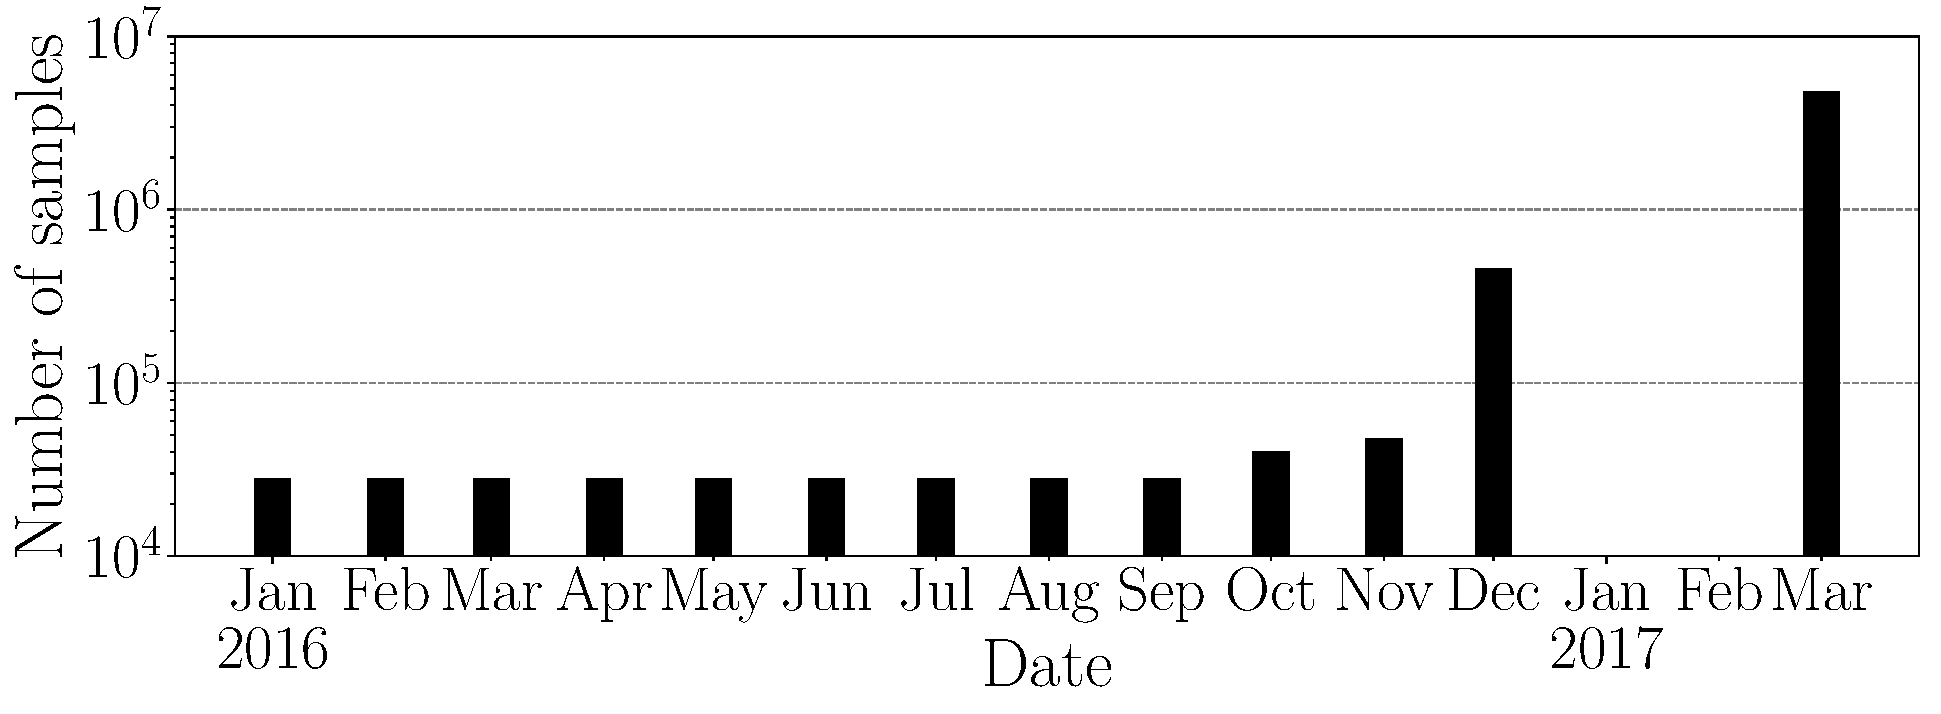
\includegraphics[width=0.8\linewidth]{time_distribution_of_customers}
    \caption[Customer distribution]{The temporal distribution of the samples.}
    \label{fig:temporal_distribution_of_samples}
\end{figure}

The customers are only represented once in this data-set. Each sample has 211 features, which are mostly numeric, but contain some categorical and ordinal fields. Features include the number of calls, data usage, network coverage, province, etc. Na\"{i}vely, one could use all the features and expand the categorical variables, producing 291 features. However, if ordinals and categorical variables are omitted (along with some features Vodafone flagged as less useful), then only 134 features remain.

\section{Resampling}

A popular approach to tackle imbalanced data is to try and \textit{rebalance} the data. This can be done by either undersampling the majority class (satisfied customers), or by oversampling the minority class (churners). Both have their pitfalls: undersampling may throw away important features in the training set, and oversampling may cause over-fitting.

A prominent algorithm for oversampling is the \textit{synthetic minority oversampling technique} (SMOTE). This takes a minority class instance, finds the samples which resemble it most closely, and generates a new synthetic sample as an interpolation of these. A close relative of SMOTE is \textit{adaptive synthetic sampling} (ADASYN), which samples frequently misclassified regions of the sample space which are deemed difficult to learn. 

To undersample the majority class, one option is to randomly remove samples. A slightly more sophisticated approach is to try to remove instances which obscure boundaries between the classes. By removing these, the boundaries should become sharper and easier to learn. One method is to remove \textit{Tomek links}. Two samples form a Tomek link if they are from different classes, and the majority instance is the closest resembling sample to the minority instance. If so, the majority instance is removed. This can be iterated several times, removing Tomek links on each parse. For the Vodafone data-set, approximately 10\% of the majority instances were removed by two parses. 

\section{Ensembles}

There are many algorithms we could use to learn from the data, each giving its own set of predictions. Furthermore, the way an algorithm learns may not be deterministic, and so the same algorithm may give different predictions over several training sessions. Multiple learners can be aggregated together to produce one overarching learner, called an \textit{ensemble}. An ensemble should have a better overall accuracy (or stability) than its constituent \textit{base learners}. We can create ensembles by \textit{boosting}, which successively introduces new learners into the ensemble based on the performance of the most recently introduced base learner. We now present two boosting variants: \textit{adaptive boosting} and \textit{gradient boosting}. 

\subsection{Adaptive boosting}


\infommmarginnote[4em]{Adaptive boosting increases the weights for misclassified samples.}
A very data-centric boosting method is adaptive boosting. The premise is to assume that several base learners have been trained and currently form an ensemble, but we want to introduce another. Taking the most recently trained learner, we see which samples from the training set it misclassifies. We then train a new learner on the same training set, but we reweight the samples. We increase the sample weights by a constant factor for those which were misclassified, and decrease those which were correctly classified. This means the new learner will increase its focus on learning those which were misclassified, and less on those which were correct. When this new learner is trained, the overall error it incurs is evaluated, and its contribution to the ensemble is weighted accordingly. The better the learner does, the greater its contribution to the ensemble. 

\subsection{Gradient boosting}


The performance of a learner can be quantified using a loss function, which measures a learner's degree of error. Traditional gradient boosting minimises this loss function using \textit{steepest descent}, numerically computing how the loss function changes if the data is slightly altered. Learning this dependency, the boosting algorithm proposes an additional learner with different parameter values in the direction it expects to reduce the loss function quickest.

\infommmarginnote[0em]{Extreme gradient boosting learns the Newton direction.}
An extension of steepest descent gradient boosting is \textit{extreme gradient boosting}. This approximates the loss function around the existing learners, incorporating corrections for curvature. Minimising the loss function's increase, the resulting learner emulates the \textit{Newton direction} of descent. An excellent implementation of extreme gradient boosting is XGBoost. 

\subsection{Cost-sensitive boosting}

Both of these boosting methods assume the loss function is equally penalised for misclassified majority instances as for minority instances. However, recalling what the samples represent, it is much worse for Vodafone if a dissatisfied customer is overlooked than if a content customer is needlessly offered a promotion. Hence the cost of these two types of misclassification is not the same. 

Different misclassification costs can be refactored into a \textit{cost-sensitive} loss function. The regular adaptive boosting algorithm AdaBoost has such a cost-sensitive extension called AdaCost. There are many ways to incorporate cost-sensitivity; we construct two new algorithms: AdaCost-B1 which is a revised AdaCost with a different error measurement, and AdaCost-AATP which penalises misclassification in the top percentiles. Furthermore, we also construct a cost sensitive loss function for gradient boosting algorithms. 

\section{Experimental results}

\subsection{Feature reduction}

The features are a mix of numeric, categorical, and ordinal values. If categorical and ordinal values are included, then there are 291 features, and only 134 if these are removed. Using XGBoost as a baseline method, we perform 15-fold cross validation. We find that the accuracies in the top \nth{5}-percentile are $ 48.5\pm 0.2 $\% using the 134 features, and $ 47.1\pm 0.4 $\% when including the ordinal and categorical variables. This implies we can use the reduced data-set, consistently achieve higher accuracies, and train algorithms faster than if we had used all the features. 

\subsection{Resampling}

To measure the efficacy of the various resampling methods, we record performances as an improvement (or reduction) relative to what XGBoost achieves without resampling. These improvements form a distribution, which we show in \Cref{fig:resampling_performance_with_xgboost}. We immediately see ADASYN gives a substantial reduction in performance. Conversely, SMOTE gives an improvement of approximately 0.3\%, although also produces an increased variance. Interestingly, removing Tomek links gives no nett improvement. 

\begin{figure}[htb]
    \centering
    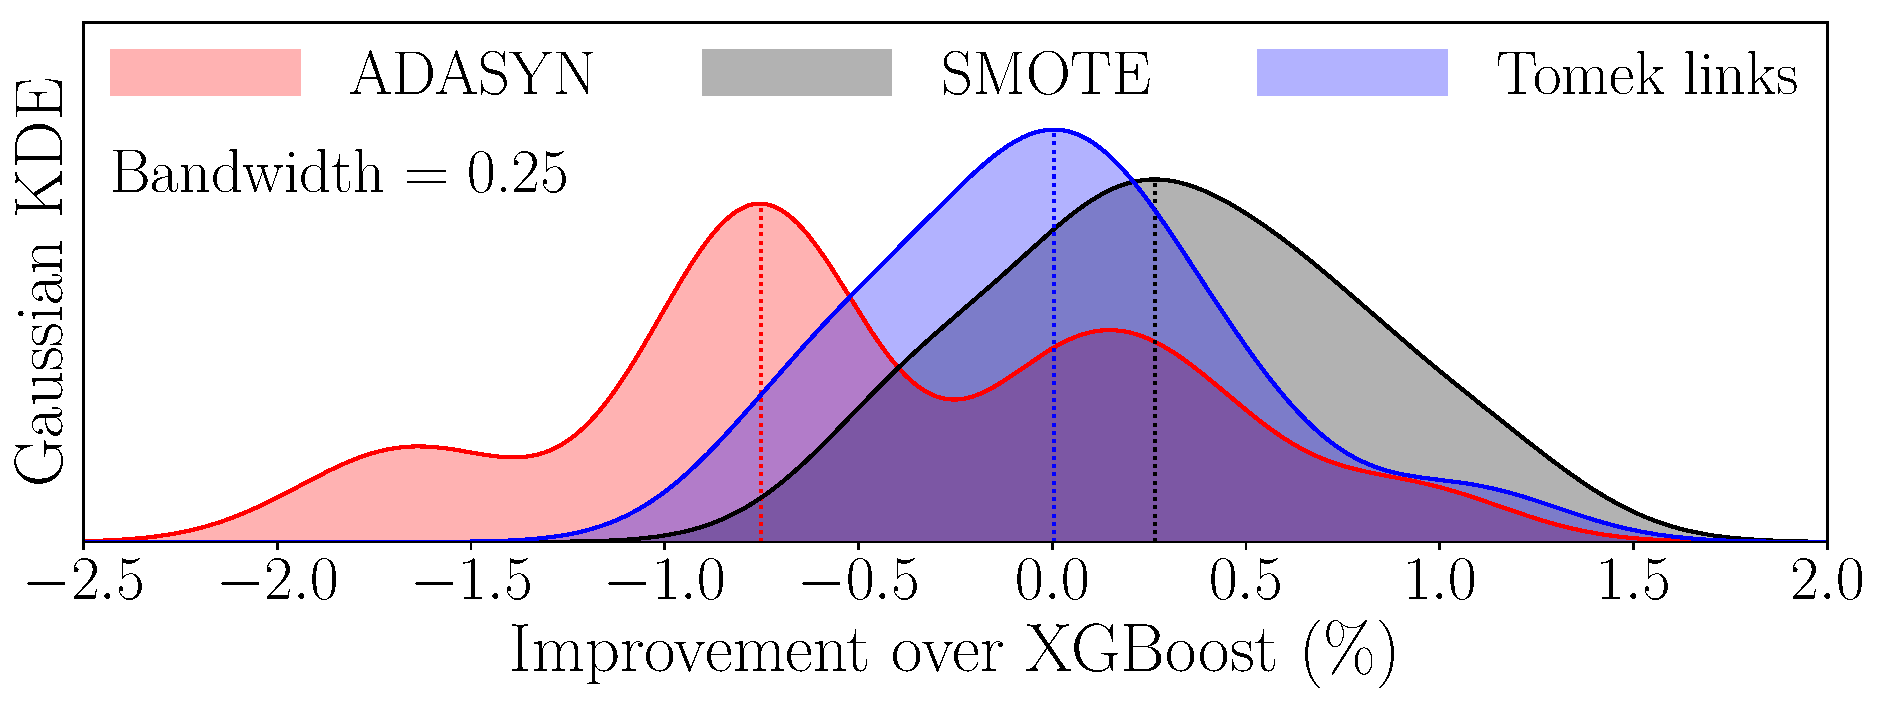
\includegraphics[width=0.8\linewidth]{top_percentile_resampling_kde}
    \caption[Resampling performance with XGBoost]{The performance gains from using various resampling methods with XGBoost.}
    \label{fig:resampling_performance_with_xgboost}
\end{figure}

\subsection{Cost-sensitive boosting}

One of our results is that AdaCost appears to show improvements above AdaBoost. In light of this, we implement balanced (and imbalanced) ensembles using random undersampling. The resulting learners were combined using either AdaBoost or the AdaCost variants. The accuracies of these algorithms for different ensembles sizes are shown in \Cref{fig:accuracies_for_cost_sensitive_random_forest_ensembles}. 

\begin{figure}[htb]
    \centering
    \infommmarginnote[5em]{Balancing the data reduced the accuracy in the top percentile.}
    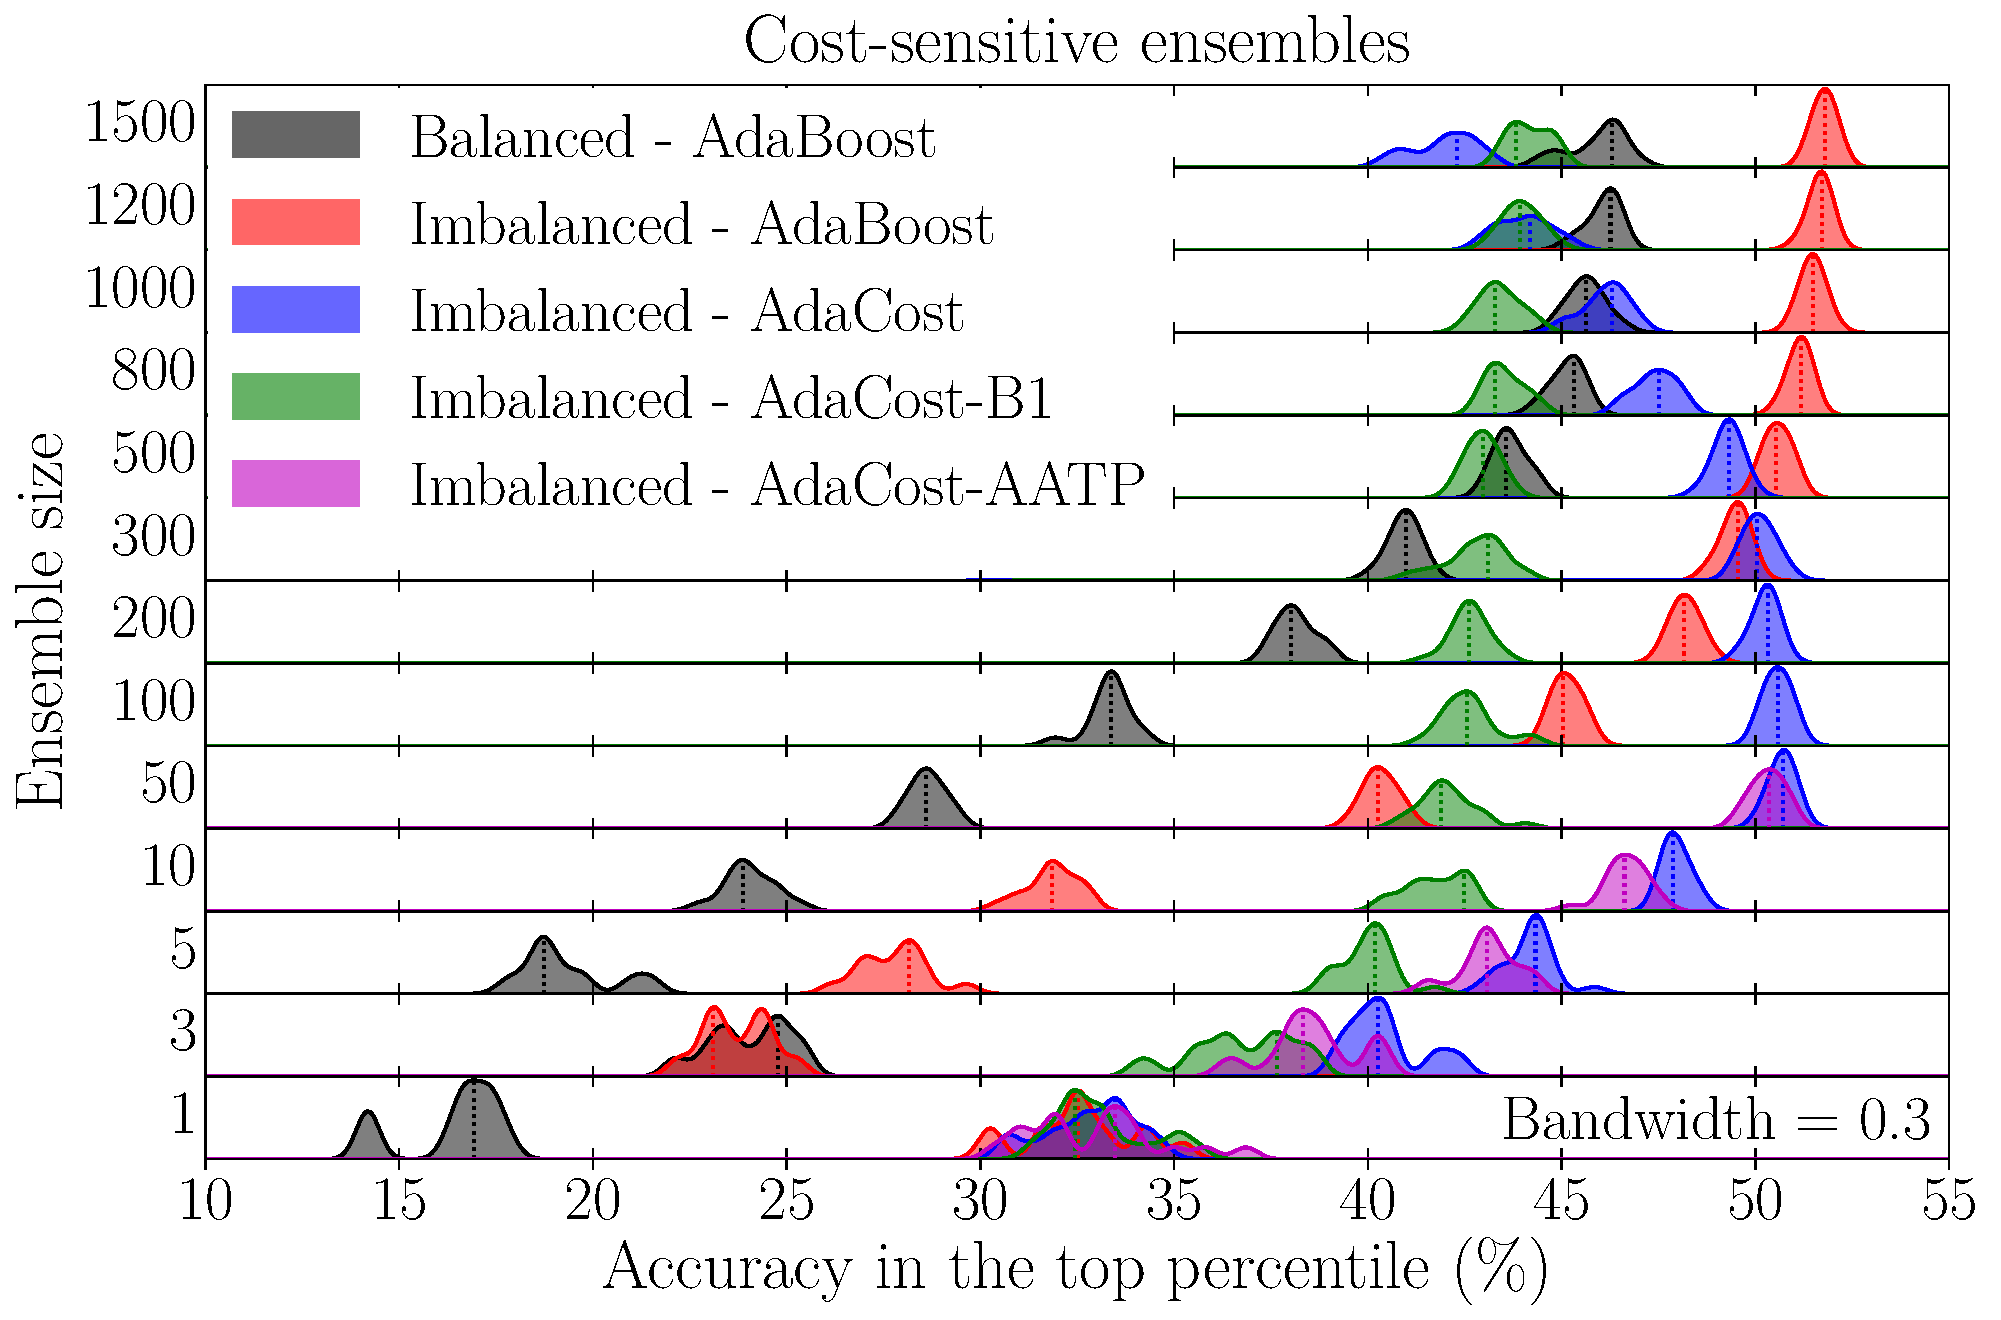
\includegraphics[width=0.8\linewidth]{balanced_and_imbalanced_random_forest_ensembles_cost_sensitive_simplified}
    \caption[Accuracies for cost-sensitive random forest ensembles]{Accuracies in the top percentile using cost-sensitive random forest ensembles.}
    \label{fig:accuracies_for_cost_sensitive_random_forest_ensembles}
\end{figure}

Several results are embedded in \Cref{fig:accuracies_for_cost_sensitive_random_forest_ensembles}. We first highlight the improvement gained when AdaBoost uses imbalanced data. This learner achieves the best accuracy across all the ensembles and algorithms we tested, with peak performance at $ 51.8\pm 0.2 $\%, which is approximately 1.5\% better than the best single algorithm Vodafone uses, and 1\% better than the accuracy they achieve from a combination of 12 different algorithms. 

The cost-sensitive boosting methods exhibit very interesting scaling with increased ensemble sizes. The most significant is that AdaCost achieved a comparably high accuracy using a much smaller ensemble size of 50. However, for larger ensembles, this performance reverted. Frustratingly, while showing promise in earlier tests, AdaCost-B1 and AdaCost-AATP did not show a competitive edge. 

We also explored cost-sensitive extreme gradient boosting, but were unable to demonstrate improved performances from introducing cost-sensitive loss functions. However, this was not exhaustive, and more work is required before dismissing this. 

\subsection{Final predictions}

After all the rounds of validation, we finally use the best performing algorithms on the final prediction set (containing 953,479 samples). We used XGBoost with and without SMOTE, and imbalanced AdaCost and AdaBoost for 50 and 1,500 base learners respectively. For comparison we also include logistic regression, (a simple case of linear models for binary classification). The accuracies achieved are show in \Cref{fig:accuracies_on_prediction_set}.

\begin{figure}[htb]
    \centering
    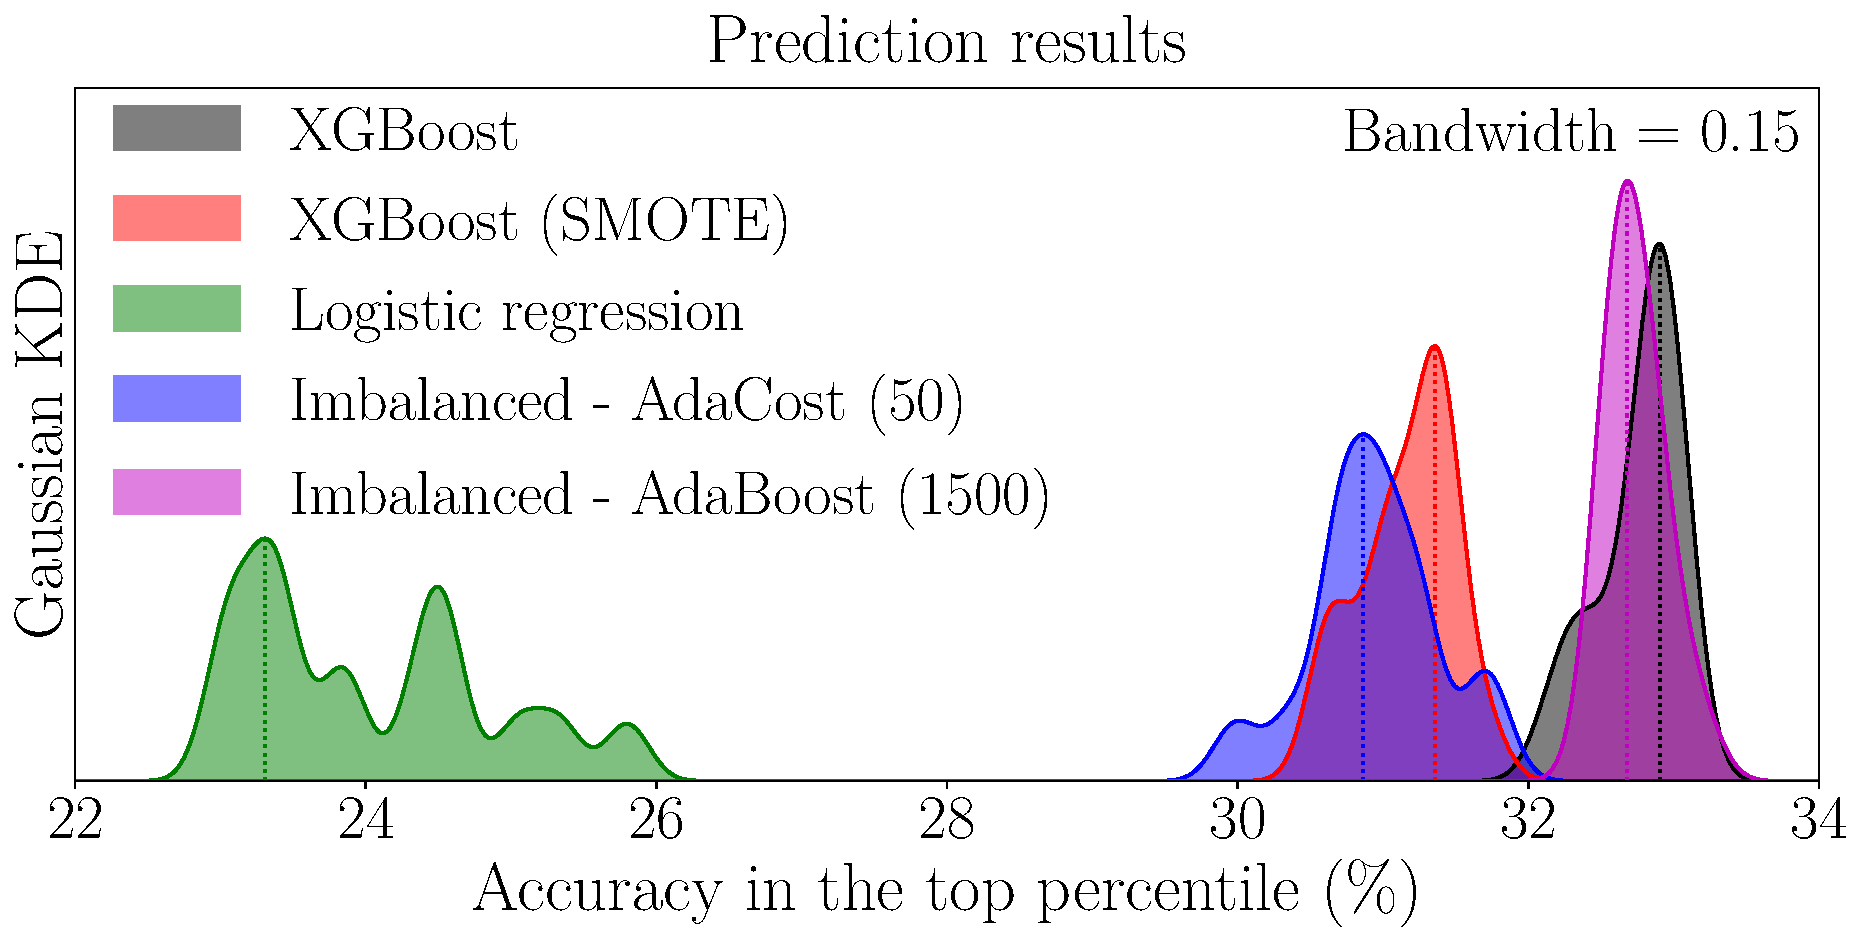
\includegraphics[width=0.8\linewidth]{predictions_simplified}
    \caption[Predictions]{The final accuracies on the prediction set. Ensemble sizes are parenthesised.}
    \label{fig:accuracies_on_prediction_set}
\end{figure}

Immediately we notice that these accuracies are all much lower than the 45--50\% expected from the validation set results.  However, given the temporal segregation of the data from \Cref{fig:temporal_distribution_of_samples}, it is not unreasonable to attribute this to an inherently more difficult data-set. We notice that XGBoost using SMOTE gives a worse performance than without, and AdaCost is appreciably worse than AdaBoost. However, AdaBoost with its imbalanced ensemble does achieve a competitive accuracy compared with XGBoost, which is as expected. Furthermore, we see AdaBoost shows a smaller variation than XGBoost.

\section{Discussion, conclusions, and recommendations}

We have considered the problem of classifying churning Vodafone customers which is a percentile herding task with an underlying data imbalance. To tackle these challenges, we have investigated data processing and feature reduction, resampling methods, and boosting algorithms. 

We inspected the data and demonstrated that higher accuracies could be achieved when using a reduced data-set. Selecting a subset of the features, ignoring the categorical and ordinal features, we reduced the number of features down from 291 to 134. The reduced set produced higher accuracies, more consistent results, and was faster and cheaper to compute. 

Within the Vodafone customer base, there is an imbalance in the number of churners and non-churners. To address this imbalance, we considered ADASYN, SMOTE, and Tomek links, which were two oversampling methods and an undersampling method respectively. SMOTE showed small but appreciable performance gains, Tomek links gave no nett improvement, and ADASYN reduced performance. Consequently, we would recommend including SMOTE in subsequent algorithm validations. 

\infommmarginnote{AdaBoost achieved an accuracy of 51.8\%.}
From the experiments with cost-sensitive boosting methods, we found a myriad of different performance behaviours. Emerging from this we found that AdaBoost, using 1,500 imbalanced base learners, achieved the highest recorded accuracy of $ 51.8\pm 0.2 $\%. This was approximately 1.5\% better than the best single algorithm Vodafone had found.

As a consequence of these findings, we would promote exploring SMOTE when developing and validating any new algorithms. Furthermore, its benefits could be realised across a wider range of algorithms. Additionally, although cost-sensitive boosting algorithms did not achieve the highest recorded accuracy, for a variety of different base learners they usually proved competitive, and would be suitable for further comparisons.

\section{Potential impact}

The challenges caused by imbalanced data, and the task of herding top percentiles, is a ubiquitous and pervasive problem frequently encountered across many areas of Vodafone's business. Having a better knowledge of approaches to tackle these difficulties, from processing the data to ensemble methods, presents many opportunities for an improved quality of service which can be passed onto Vodafone's customers. 

\begin{myquote}[Dr Uwe Bombosch\\Lead data scientist at Vodafone Germany]
Finding a top quantile with a high true positive rate is a ubiquitous problem in our business, in fact more wide-spread than a good overall classification. The outcome of the InFoMM mini-project can immediately be applied to several machine learning models we are building for marketing and customer satisfaction campaigns. SMOTE, for instance, has already found its way into a campaign channel optimisation. In addition to the insights, we also received a package of well-written code for our toolbox. When applying for a mini-project, I expected the highest level of maths, but was surprised by the IT-literacy and the hands-on approach. I clearly recommend InFoMM projects as a source of inspiration to data science organisations.
\end{myquote}

\clearpage
\end{document}












